\documentclass[letterpaper,sansserif,tightsqueeze]{rpg-module}

\usepackage{parskip}                                                            % Add spacing between paras instead of indents
\usepackage[font=bf]{caption}

\title{W1: Dungeons and Dragons?}

% Compress title spacing compared to default

\addtolength{\topmargin}{-0.3cm}
\addtolength{\textheight}{0.7cm}

% Initialise counters

\setcounter{page}{20}
% Type|Asterisk for special weapon|AC|HD|MV/T|MV/R|spcial move|SMV/T|SPM/R|Attack|attack desc.|dmg|dmg long|ST|alignment|No. appearing|No. in lair|treasure|XP
%\monster[Shrukk]{shrukk}{Shrukk}{||5|4+1|30'|9||||1 weapon|Weapon|1d10|1d10|13|C|1|1|Nil|120}
%\monster[Human Berserker]{human_berserker}{Human Berserker}{||7|1|40'|12||||1 Weapon|Weapon|1d8|1d8|17|C|1--5|1--5|Nil|30}
%\monster[Gnoll]{gnoll}{Gnoll}{||5|2|30'|9||||1 Bite or 1 Weapon|Bite or Weapon|2d4 or 1d10|2d4 (bite) or 1d10 (weapon)|16|C|1--6|1--6|Nil|30}
%\monster[Vampire Bat]{vampire_bat}{Vampire Bat}{||8|1|13'|4|Fly|60'|18|1 Bite|Bite|1d6+special|1d6\+blood drain|17|N|1--3|1--3|Nil|60}
%\monster[Piercer]{piercer_1hd}{Piercer}{||3|1|3'|1||||1 Drop/Pierce|Drop/Pierce|1d6|1d6|14|N|1|1|Nil|15}
%\monster[Piercer]{piercer_3hd}{Piercer}{||3|3|3'|1||||1 Drop/Pierce|Drop/Pierce|3d6|3d6|14|N|1|1|Nil|60}
%\monster[Wolf]{wolf}{Wolf}{||7|2+2|60'|18||||1 Bite|Bite|1d4+1|1d4+1|16|N|1|1|Nil|30}
%\monster[Goat]{goat}{Goat}{||8|1|30'|9||||1 Head-butt|Head-butt|1d4|1d4|18|N|1|1|Nil|15}
%\monster[Giant Centipede (non--lethal)]{giant_centipede}{Giant Centipede (non--lethal)}{||9|1d2|43'|13||||1 Bite|Bite|special|special|18|N|2d12|0|Nil|15}

% \monster{vampire_bat}{Giant Vampire Bat}{Bat||6|2|30'|10'|Fly|180'|60'|1|1 bite|1d4+special|1d4\+blood drain|Fighter: 1|8|Neutral|1--10|1--10|Nil|20}

\begin{document}

\twocolumn

\title{Dungeon Module W1\\
	Dungeons and Dragons?}

\subtitle{An Adventure for Character Levels 2-4...I guess}

%\coverimage{dragon-cover.jpg}
\coverimage{dragon.png}

\abstract{Seeking treasure and the lair of Cadmus the Destroyer, you find yourself on the top of a hill. Will you be able to stop Cadmus once again and restore the peace that held for a hundred years? 
	
	This module contains referee notes, background information, maps, and exploration keys intended for
	use with the Old-School Essentials rules. Be sure to look for other OSE modules from Necrotic Gnome.}


\maketitle

\onecolumninline{\part*{LEVEL 1: The entrance to the dungeon}}

\section{Introduction}
The adventurers have been briefed about a dragon holding up in a nearby dungeon, long perceived as abandoned. Did Cadmus the Destroyer return?

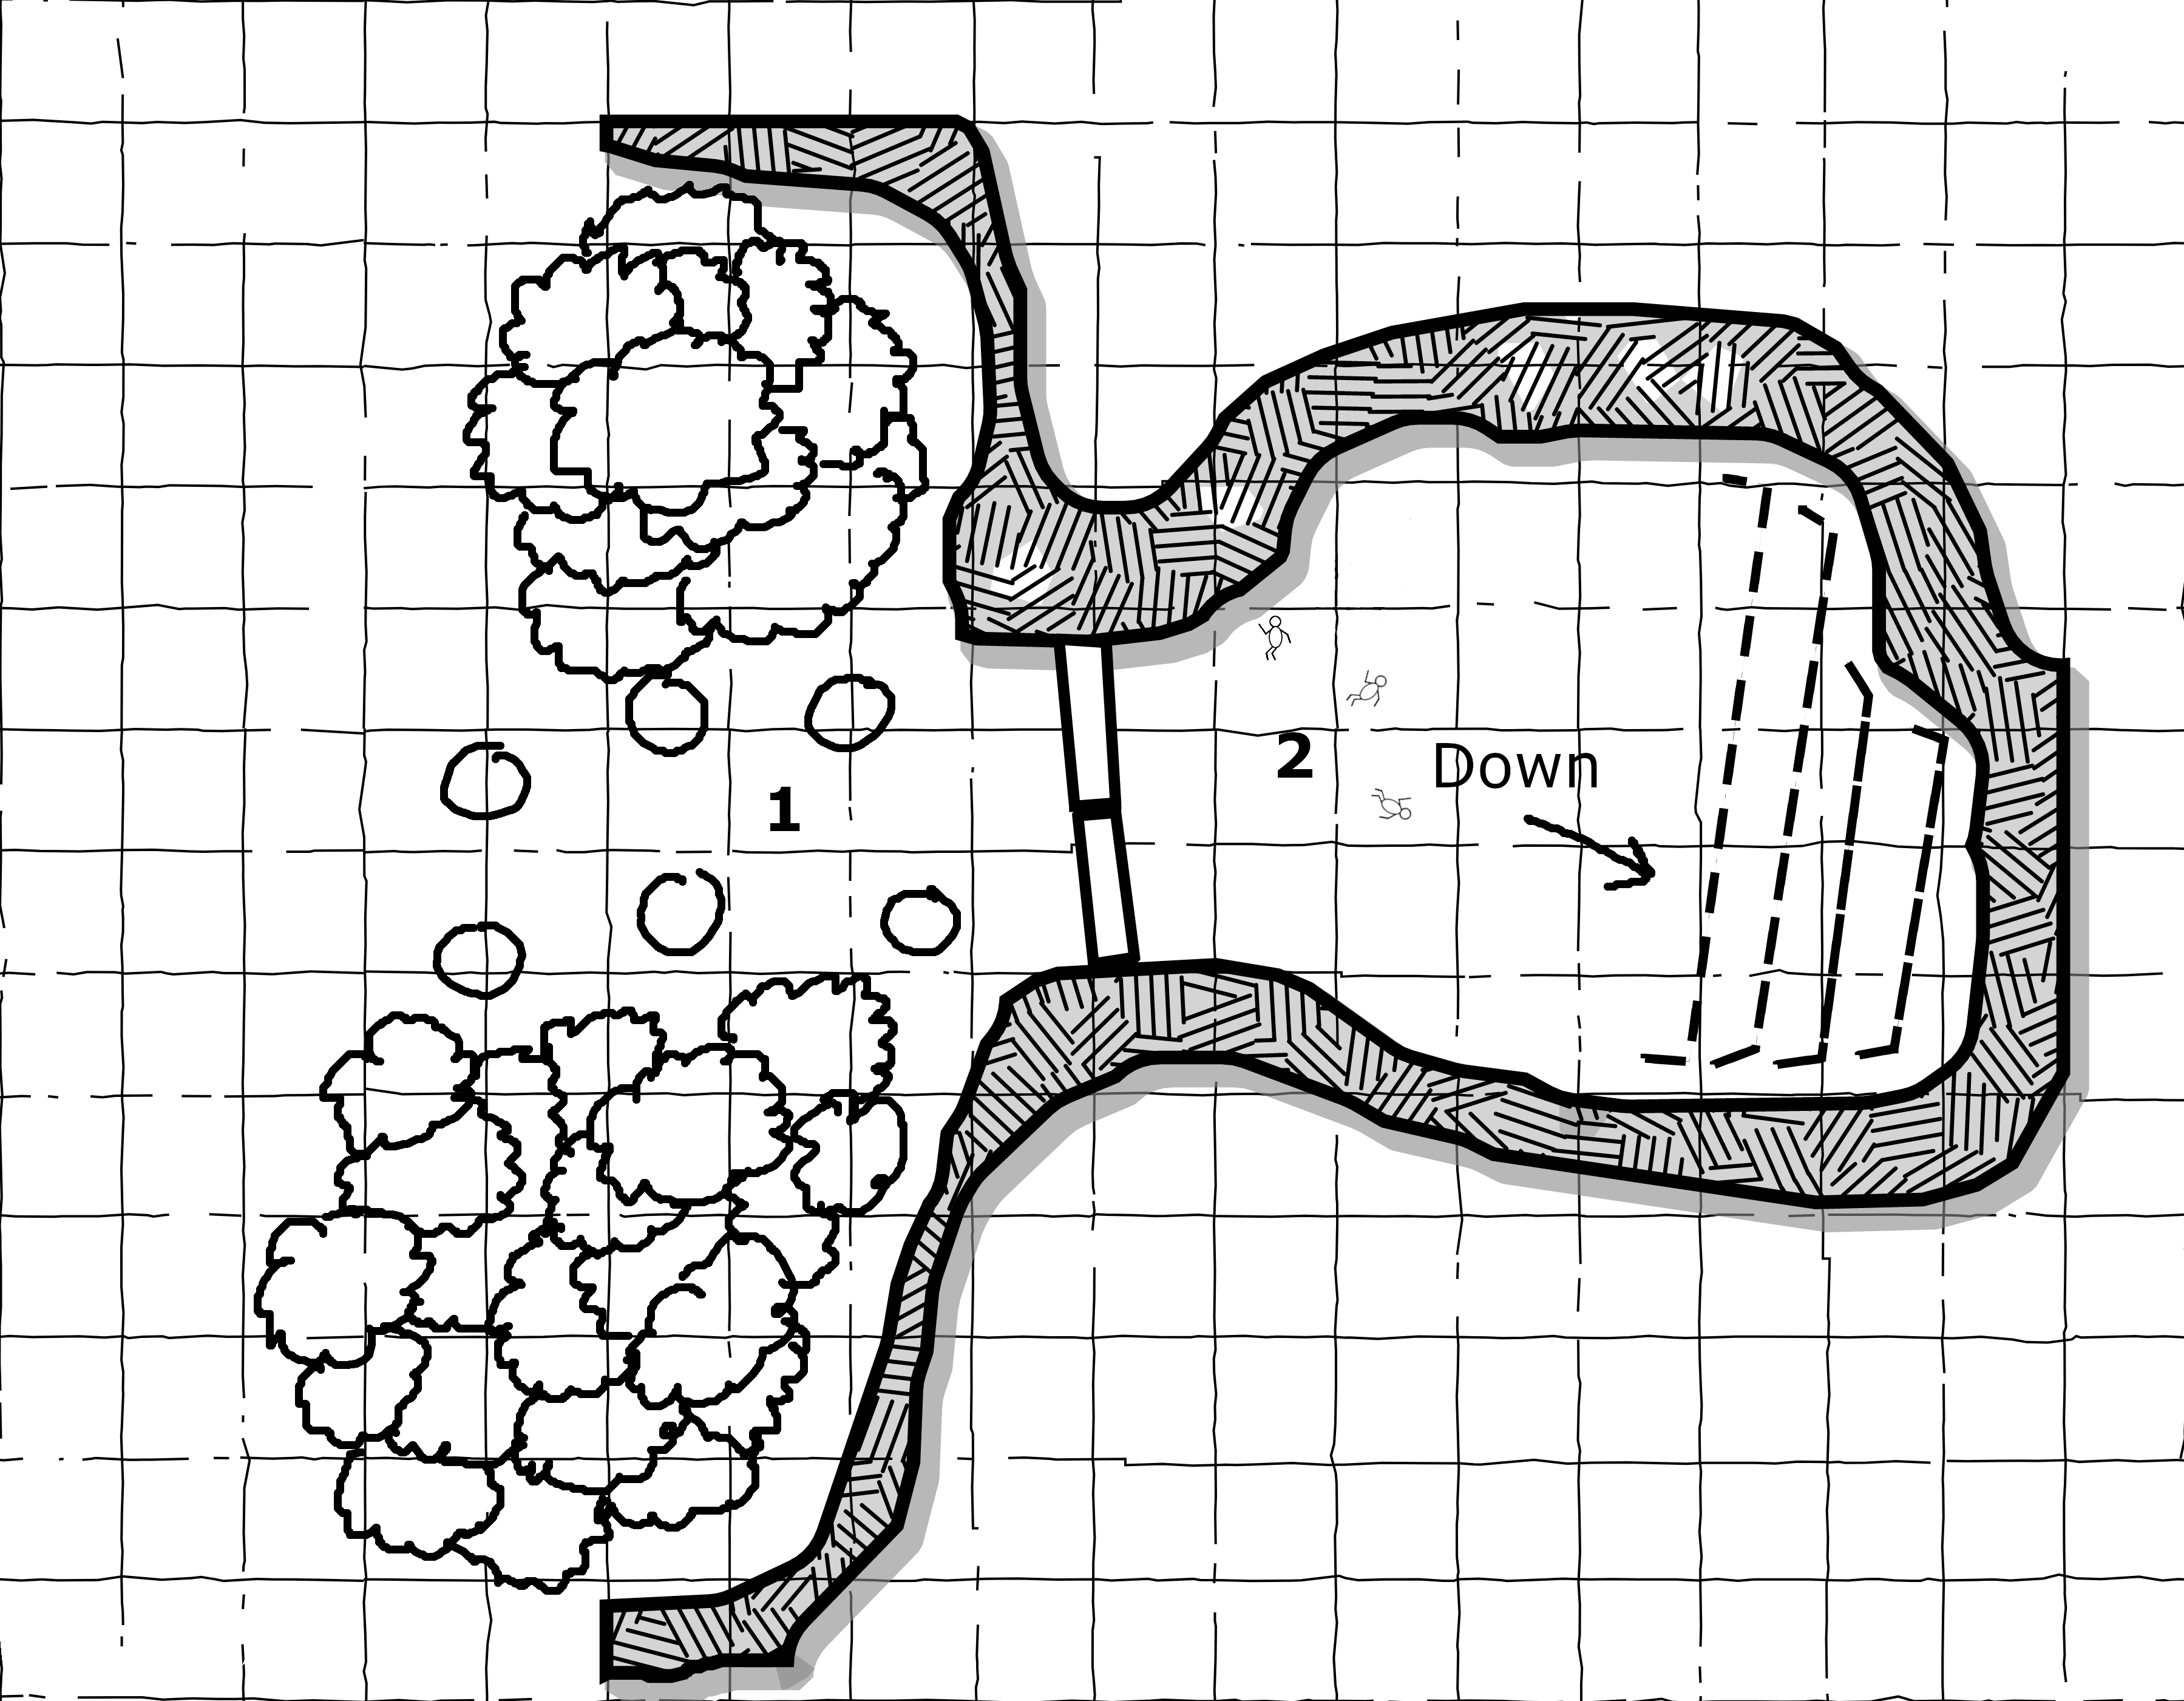
\includegraphics[width=\linewidth]{map_secret_1.png}

\vspace{0.2cm}

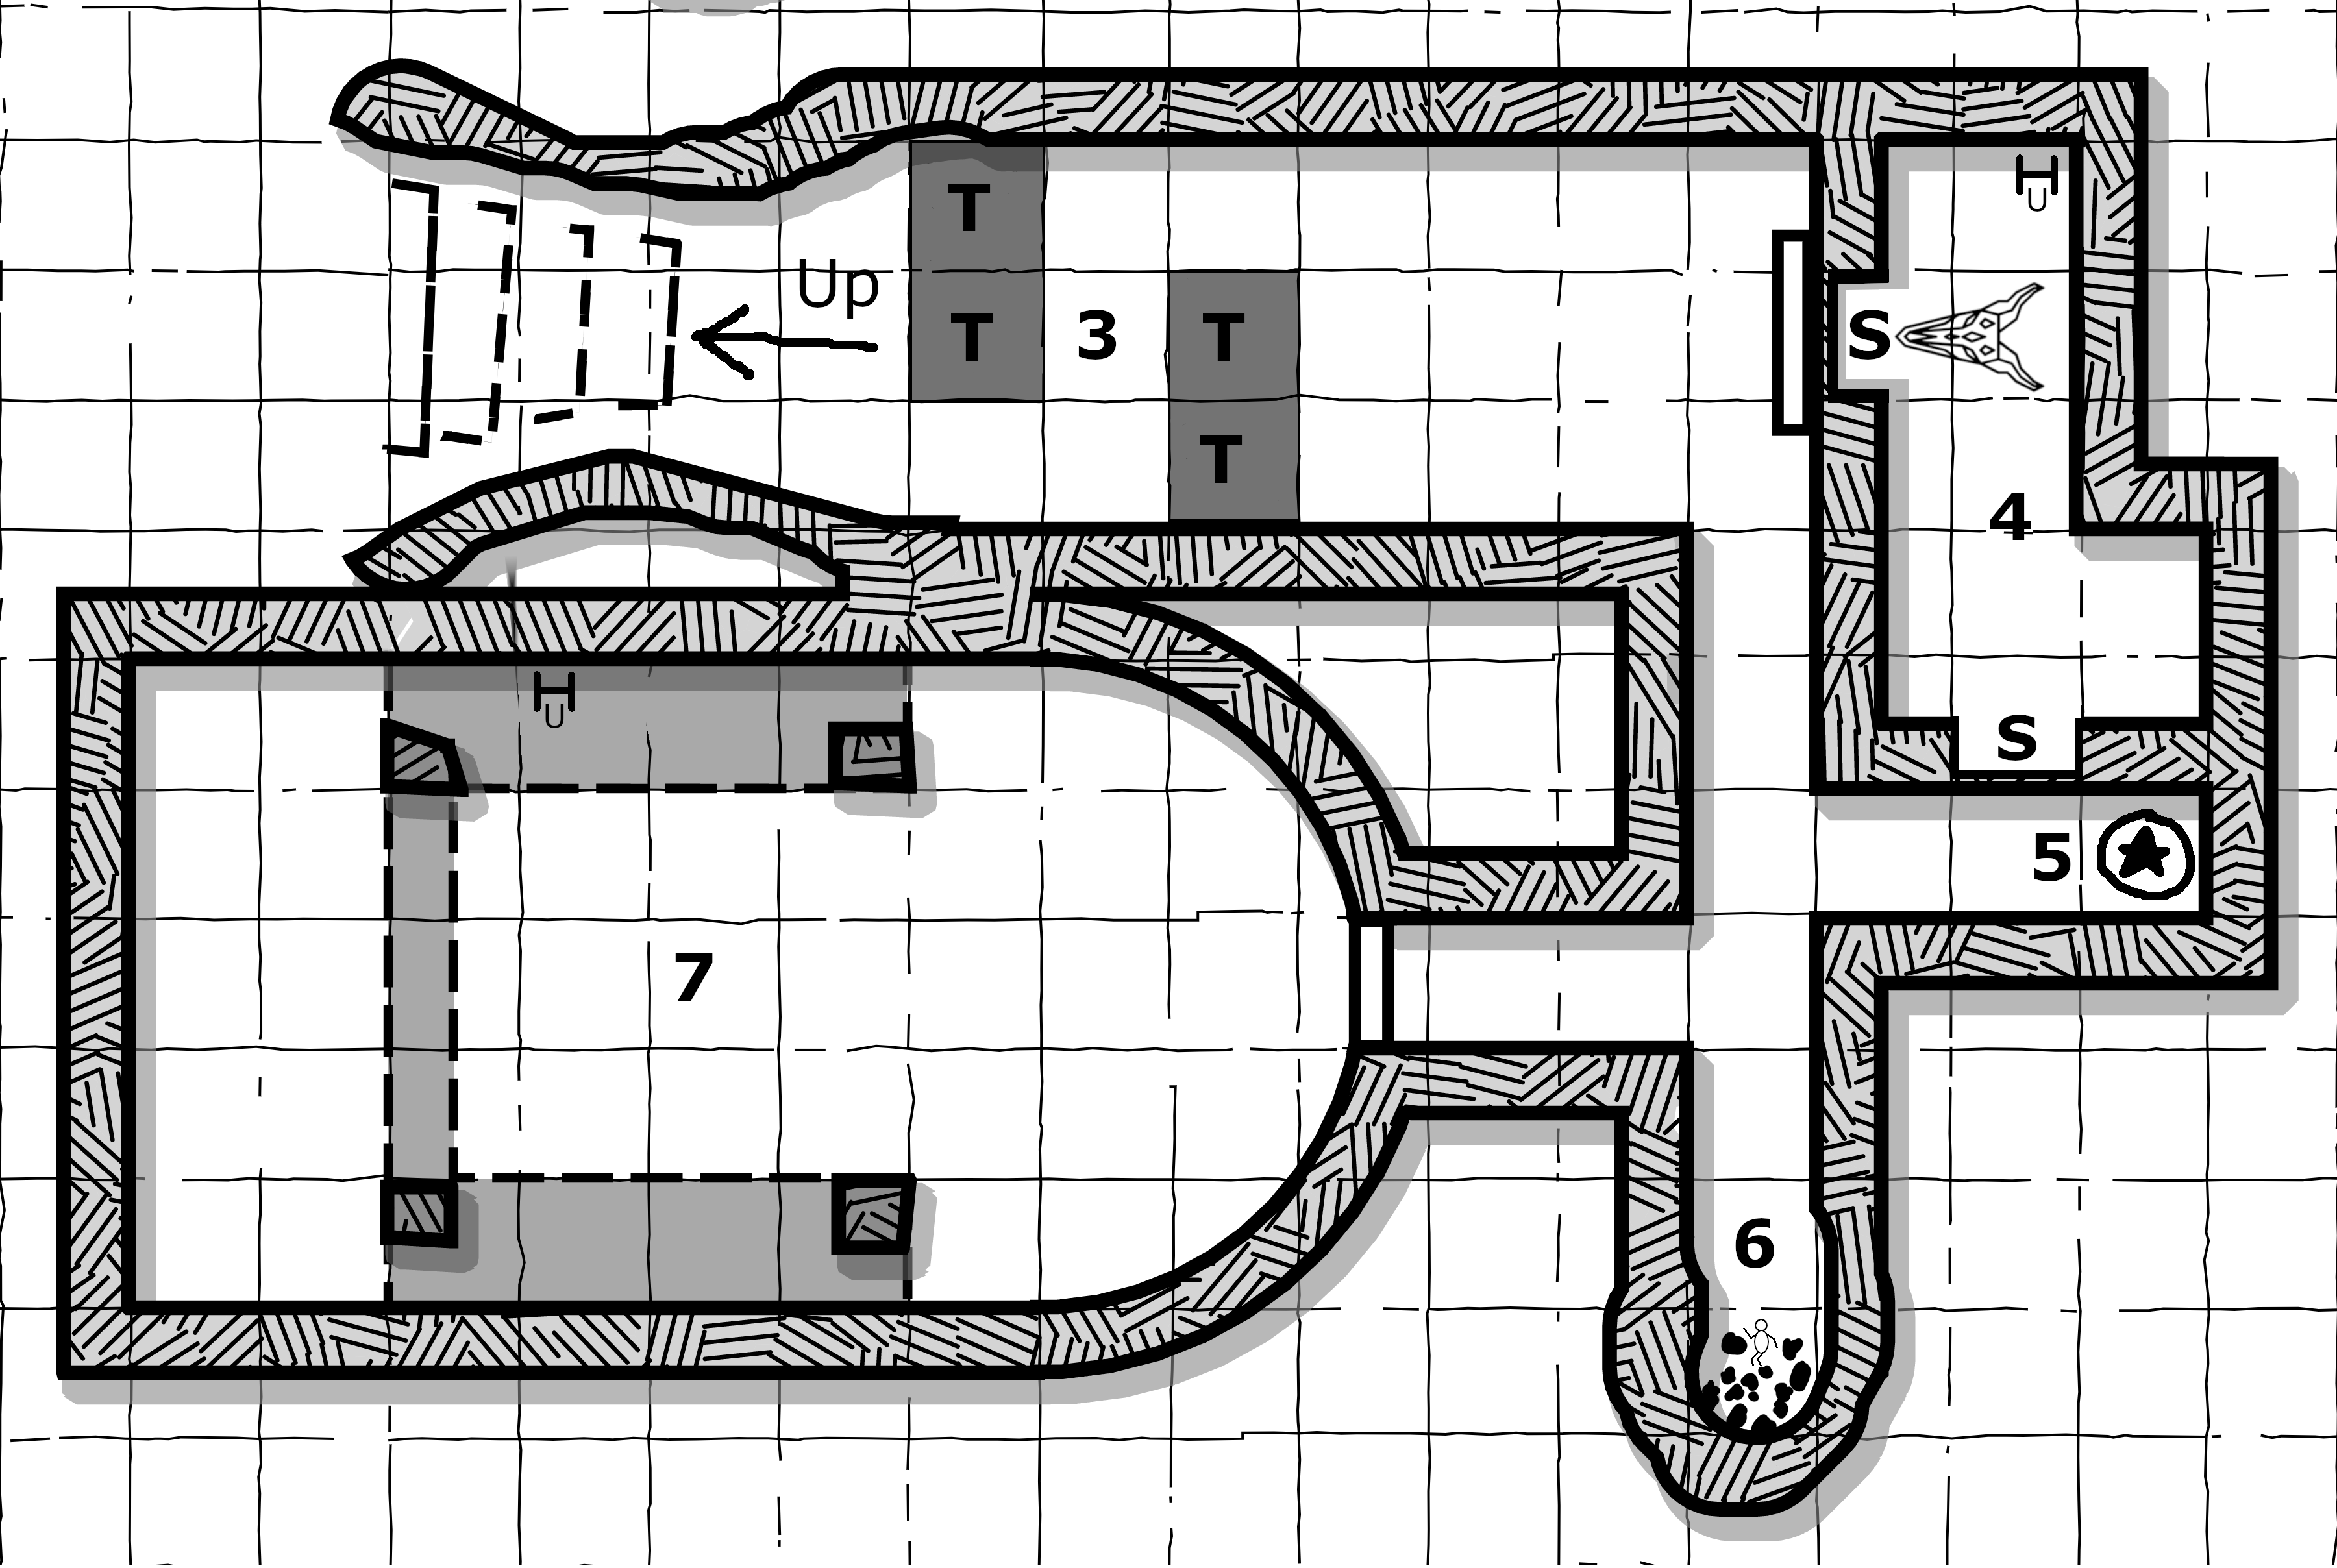
\includegraphics[width=\linewidth]{map_secret_2.png}

\section{1-2. THE ENTRANCE}

\setcounter{subsection}{0}

\subsection{MOUNTAIN-SIDE}
\textit{Cut down trees form a path. Two large wooden doors, above these doors something is written in green luminescent ink. The smell of freshly cut wood. \textbf{Hidden: Small (kobold) footprints}}

The party starts at the entrance of a cave.

\begin{boxtext}
	After a half day's worth of travelling you find yourself at an opening in the hill-side forests, this opening seems man-made the trees were cut down to knee-high stumps. One of the villagers takes a step forward "This should be it, Cadmus is hiding behind that door". Two large doors sit in the side of the hill, above the doors you see runes written in a luminescent green ink.
\end{boxtext}

The runes were written by kobolds and should function as a warding spell that triggers if the doors are opened one at a time. However, due to its amateurish execution the spell only sizzles when triggered. 

\textbf{Treasure:} Two (unused) torches lie near the doors.

\subsection{THE NATURAL STAIRS}
\textit{4 lifeless bodies lie on the floor, the victims' clothes are charred.}

The bodies on the floor belong to a previous group of adventurers that tried to find Cadmus, they were at the receiving end of the fire cannon hidden in room 4. Roll on table \ref{tab:search_body} to discover what is found when searching the bodies.

\section{3-6. CADMUS' LAIR}

\setcounter{subsection}{2}

\subsection{HALL}
\textit{Smell of blood. Floor cleaned recently, but residue of oil remains on the northern wall.}

This hall in unlit at the eastern end of the hall a life-size portrait of Cadmus in his human-form is visible.

The hall has been trapped with pressure plates that release the stalactites on the ceiling.

\subsection{SECRET WATCHPOST}
\textit{Smell of sweat mixed with lamp oil. A ladder leads upward \textbf{Hidden: A small metal tab on the western walls hides a peak hole.}}

A small metal tab hides a peak hole and a larger door can be opened to allow weapons to be fired through the Cadmus painting. A small ladder at the northern end of the room leads up to a secret escape route. A dragon head-shaped cannon that fires fireballs is present in this room.

\subsection{CADMUS' STATUE}
\textit{A statue in pristine state, otherwise dusty floors. Statue is hiding its eyes behind its hands.}

The statue's hands can be lowered to reveal the secret door in the southern wall of room 4.

\subsection{CAVED HALL}
\textit{High-pitched screeches can be heard under and behind the rubble, the dust has settled.}

This hall lead to the make-shift messroom of the Kobold clan, but all that remains is rubble.

\subsection{AUTONOMOUS LAB}
\textit{Mechanical whirs can be heard, the room is filled with tables full of alchemical experiments. Grappling arms whizz around. Noticeably warmer that the other rooms in the dungeon. A 10-ft high balcony \textbf{Hidden: A secret hatch hidden under tables in the center of the room containing a mechanical dragon}}

The former throne room of Cadmus the Wizard, turned into an autonomous laboratory.

The laboratory is filled with crates, tables full of alchemical concoctions, and active grappling arms. The laboratory has a X-in-6 chance of being triggered any time a character moves more than one square, X = number of squares - 1. Chance of triggering an effect is doubled when no light source is present. Roll on table \ref{tab:laboratory_events} whenever a random event occurs.

Monsters: 4d4 kobolds, busy working on alchemical weapons and fuel for the mechanical dragon, the kobold Chieftain sits on his throne near the western wall, next to the panel used for opening/closing the floor and ceiling hatches. Two of the kobolds are stationed on the balcony (dashed lines).

After 1d4 rounds the floor and ceiling hatches will have opened, 1d4 rounds later the mechanical dragon (see \textit{Monsters}) will be manned and activated.

\part*{Tables}
\begin{table}[h]
	\caption{Searching a body}
	\label{tab:search_body}
	\begin{tabular}{p{0.1\linewidth} | p{0.85\linewidth}}
		\textbf{d12} 	& \textbf{Event} \\ \hline
		1				& A torn and burned bandana. \\ \hline
		2				& A dagger smeared with a thick fluid, some of it survived the flames. \\ \hline
		3				& A half-burned picture, seems to depict one of the female farmers you saw deeply in love in the town square. \\ \hline
		4				& 1d6 copper pieces. \\ \hline
		5				& A backpack containing a tent which directly unfolds on removal, you can't seem to get it back into the backpack. \\ \hline
		6				& A quest log: 15 gold for Cadmus' head. \\ \hline
		7				& A climber's kit. \\ \hline
		8				& A torch that is still lit, strange that you didn't notice this earlier. \\ \hline
		9				& A 1st level magical wand, but a single charge remains. Screams loudly when fired. \\ \hline
		10				& A pin depicting a slain dragon, worth 1 silver. \\ \hline
		11				& A pouch of ball bearings. \\ \hline
		12				& The body reacts, you just got yourself a possible retainer. Only 1 HP remains from his/her 4 HP total. Roll an NPC reaction check (2d6): \\
		& \textbf{2 or less:} Hostile, attacks \\
		& \textbf{3 - 5:} Unfriendly, may attack \\
		& \textbf{6 - 8:} Neutral, uncertain \\
		& \textbf{9 - 11:} Indifferent, uninterested \\
		& \textbf{12+:} Friendly, helpful
	\end{tabular}
\end{table}

\begin{table}[h]
	\caption{Random laboratory events}
	\label{tab:laboratory_events}
	\begin{tabular}{p{0.1\linewidth} | p{0.85\linewidth}}
		\textbf{d6}		& \textbf{Event} \\ \hline
		1				& \textbf{You trip:} Any and all carried alchemical bombs are triggered. \\ \hline
		2				& \textbf{The fire prevention system is tripped:} All torches are snuffed out. \\ \hline
		3				& \textbf{You accidentally trigger a floor switch:} Nothing happens...absolutely nothing. Roll 1d4 to see how many rounds from now nothing will happen. \\ \hline
		4				& \textbf{You slip...:} A clockwork Goblin - triggered by your scream - erupts from one of the walls which starts to attack a nearby character: *Roll 1d4 to discover where the clockwork Goblin appears (1 = North, 2 = East, 3 = South, 4 = West). \\ \hline
		5				& \textbf{You are grabbed by a grappling arm:} Roll 1d6: \\
						& \textbf{1.} Moved 1d6 x 5 ft. to the north. \\
						& \textbf{2.} Moved 1d6 x 5 ft. to the east. \\
						& \textbf{3.} Moved 1d6 x 5 ft. to the south. \\
						& \textbf{4.} Moved 1d6 x 5 ft. to the west. \\
						& \textbf{5.} You are grabbed and packed in a crate: +1 AC, but movement limited to 5 ft/round. Need help to doff this "armor". \\
						& \textbf{6.} The grappling arm goes haywire causing all adjacent creatures to fall to the ground. \\ \hline
		6				& \textbf{You knock a bottle from the nearest table:} All squares you crossed catch fire, excluding the square you ended on. The fire extents to all adjacent squares at the start of each next round. Fire can be quenched by triggering the fire prevention system.
	\end{tabular}
\end{table}

\newpage
\part*{Monsters}
\textbf{Clockwork Goblin}
Small, mechanical contraptions representing goblins with metallic skin and glowing, red eyes. Can burrow through walls and floors.

\textbf{AC} 6 [13], \textbf{HD} 1-1, \textbf{Att} 1x weapon (1d6 or by weapon), \textbf{THAC0} 19 [0], \textbf{MV} 60' (20'), \textbf{SV} D14 W15 P16 B17 S18 (NH), \textbf{ML} 7 (9 with king), \textbf{AL} Chaotic, \textbf{XP} 5 (bodyguard: 20, king: 35), \textbf{NA} 2d4 (6d10), \textbf{TT} R (C)
\begin{itemize}
	\item \textbf{Infravision:} 90'.
	\item \textbf{Build to hate dwarves:} Attack on sight.
	\item \textbf{Build in batches:} 2d4 2HD (2d6hp) Clockwork Goblins are created in one go.
\end{itemize}


\textbf{Kobold}
Small, wicked, hairless, canine humanoids with scaly, rust-coloured skin. Dwell underground.

\textbf{AC} 7 [12], \textbf{HD} 1/2, \textbf{Att} 1x weapon (1d4 or by weapon -1), \textbf{THAC0} 19 [0], \textbf{MV} 60' (20'), \textbf{SV} D14 W15 P16 B17 S18 (NH), \textbf{ML} 6 (8 with chieftain), \textbf{AL} Chaotic, \textbf{XP} 5 (bodyguard: 15, chieftain: 20), \textbf{NA} 4d4 (6d10), \textbf{TT} P (J)
\begin{itemize}
	\item \textbf{Ambush:} Set up surprise attacks.
	\item \textbf{Infravision:} 90'.
	\item \textbf{Hate gnomes:} Attack on sight.
	\item \textbf{Chieftain and bodyguards:} A 2HD (9hp) chieftain and 1d6+1 1+1HD (6hp) bodyguards live in the kobold lair.
	\item \textbf{Hoard:} Only have treasure type J when encountered in the wilderness or in their lair.
\end{itemize}


\textbf{Mechanical Dragon (stats should not be needed)}
Gigantic, mechanical contraption representing a golden dragon fitted with an oil reservoir and a small kobold-sized cockpit.

\textbf{AC} -3 [21], \textbf{HD} 11** (49hp), \textbf{Att} [2x claw (2d4), 1x bite (6d6)] or breath, \textbf{THAC0} 11 [+8], \textbf{MV} 90' (30')/240'(80') flying, \textbf{SV} D6 W7 P8 B8 S10 (11), \textbf{ML} 10, \textbf{AL} Lawful, \textbf{XP} 2700 , \textbf{NA} 1d4 (1d4), \textbf{TT} H
\begin{itemize}
	\item \textbf{Attack pattern:} Typical order of operation: attack first with its breath weapon, then either breath again or make a melee attack (equal chance of either).
	\item \textbf{Breath weapon:} Can be used up to three times per day. All caught in the area suffer damage equal to the dragon’s current hit points (save versus breath for half). Shapes of breath weapon:
		\subitem \textbf{Cloud:} 50' long, 40' wide, 20' high.
		\subitem \textbf{Cone:} 2' wide at the mouth, 30’ wide at far end.
		\subitem \textbf{Line:} 5' wide along whole length.
	\item \textbf{Heat shielding:} Unharmed by its own breath weapon or lesser versions thereof. Automatically save versus similar attack forms.
\end{itemize}

\begin{itemize}
	\item \textbf{Ambush:} Set up surprise attacks.
	\item \textbf{Infravision:} 90'.
	\item \textbf{Hate gnomes:} Attack on sight.
	\item \textbf{Chieftain and bodyguards:} A 2HD (9hp) chieftain and 1d6+1 1+1HD (6hp) bodyguards live in the kobold lair.
	\item \textbf{Hoard:} Only have treasure type J when encountered in the wilderness or in their lair.
\end{itemize}

% Monster:
% 
% Treasure \& Location:
% 
% \subsection{GRAND CAVERN OF THE BATS}
% This majestic cave is the
% largest in the complex, and is impressive due to its size and
% volume, for the ceiling is almost 60' above. A corridor sloping
% downward into the cavern (noticeable even by nondwarves)
% gives primary access to the room on its south wall.
% A secondary entrance/exit is via a secret door to the west,
% while steps to the southeast lead up to room 52.

\end{document}
